\begin{figure}[h]

\centering
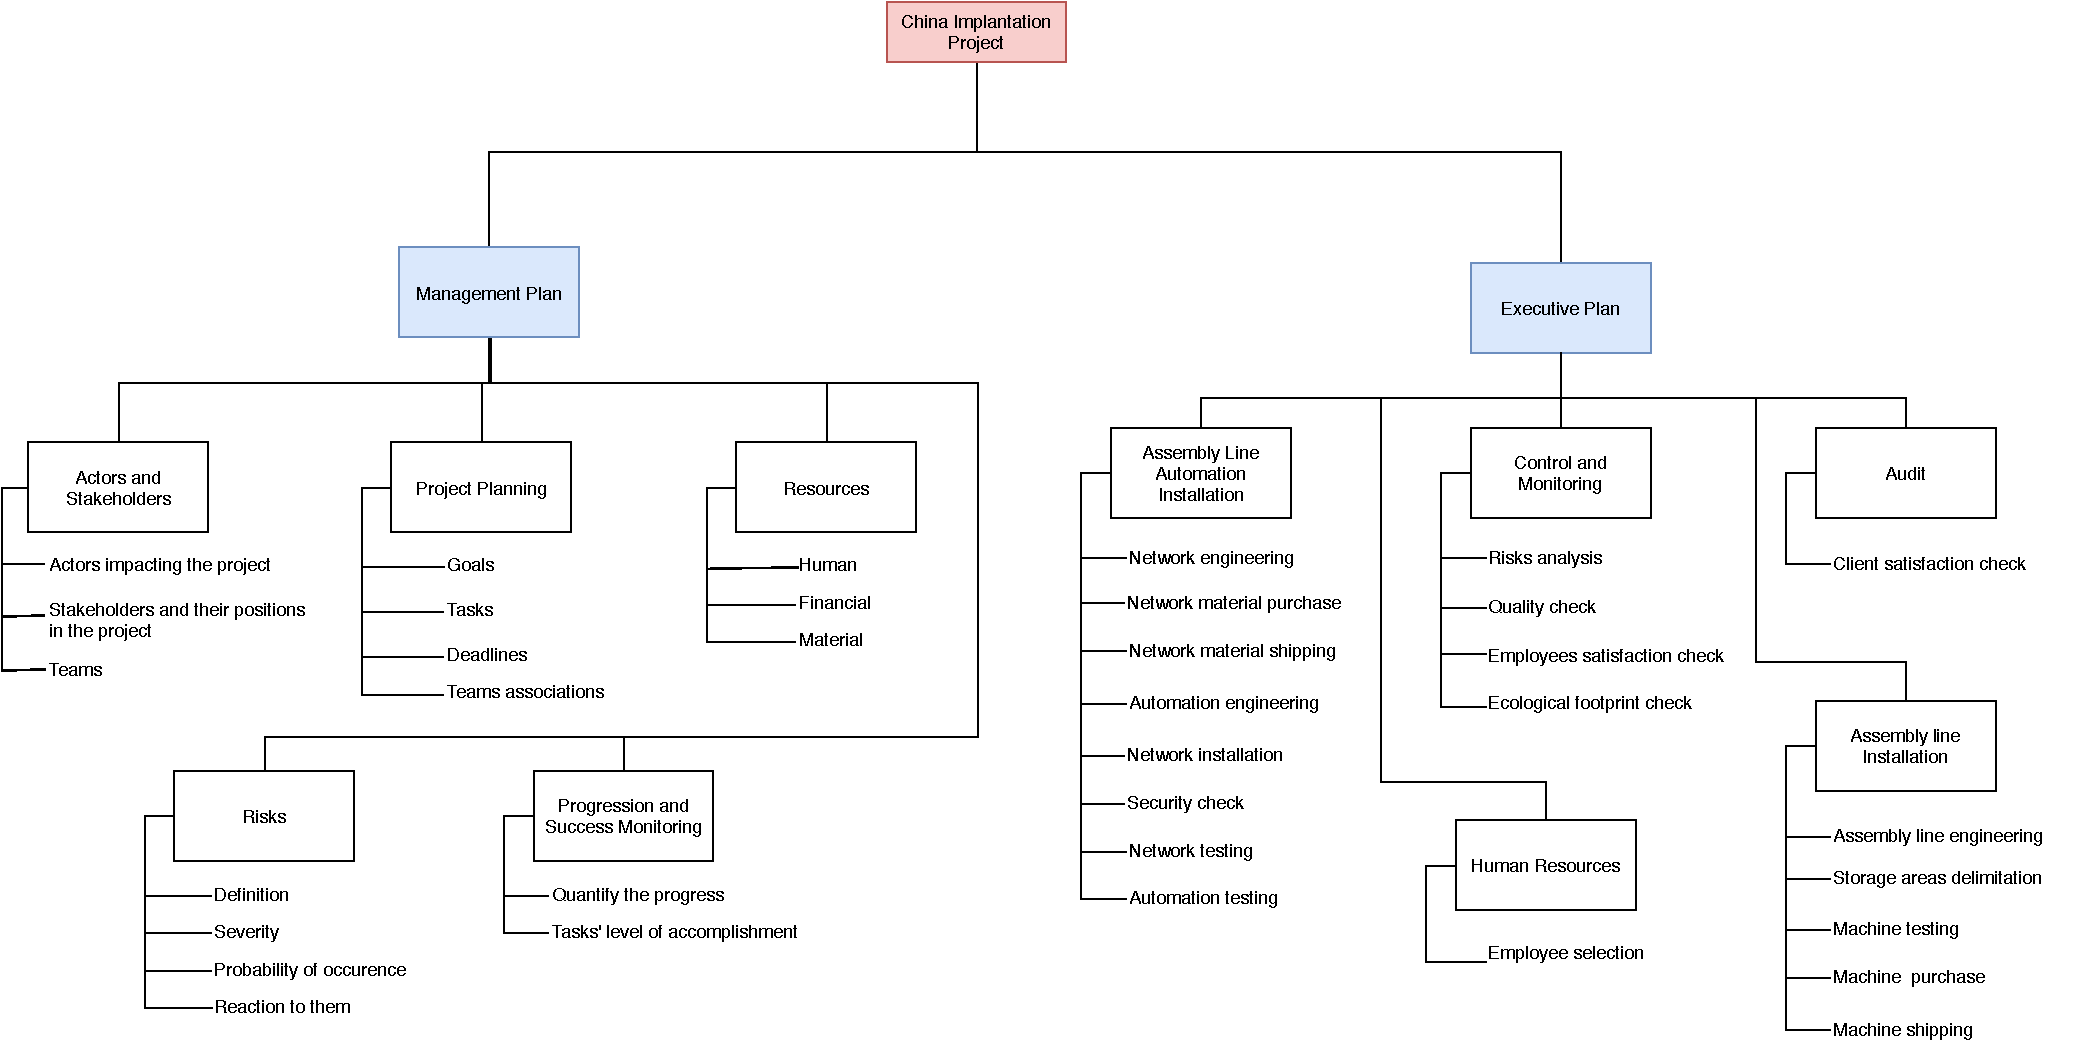
\includegraphics[scale=0.5]{Img/wbs-management-inter.pdf}
\caption{Work Breakdown Structure of the project}

\end{figure}

\subsection{Tasks}

The project is separated in many tasks that represents all steps needed to reach the goal of the project.
These tasks are separated in two categories : \emph{Managment plan} in which all the tasks represents the redaction od the management plan of the project and \emph{Executive plan} the represent the active part of the project in which the assembly line is installed.

\subsubsection{Management Plan}

The management plan is the part in which each step of the project is defined.
The management plan is defined as a frame for the project and theses tasks must be achieved before all executive task.
This part begins with a precise description of the project and goals followed by the 5 next parts.

\paragraph{Actors and Steakholders} In this parts, we must think and describe all the avtors involved in the project.
These actors are steakholders and can interact in some way with the project.
The description includes theire position, their importance and the manner that they interact with the project.
This task have also a goal of definition different teams that are required to bring this project to life.

\paragraph{Project planning} Within this task, we must think and describe all the tasks required to finish the full project, the time and resources required to achieve each task and what are task dependencies.
In this task, we must define what are deadlines and when to make debreiefing and evaluate the progression of the project.

\paragraph{Resources} In this part of the project, we must identify and write the required resources to achieve each task defined in the \emph{Project planning} part.
These resources include : human resources, financial resources and material resources.

\paragraph{Risks} In this task, we must define the primary risks that can occur during the project and how to reduce the side effect of each risk.
Each risk have a severity and prbabilty rate that represent the criticity of it.
Higher the criticity is, important the risk must be and planned with caution.

\paragraph{Progression and success monitoring} Finally, in the progression monitoring we must identify what indicator can represent the progression or the success of each task and the whole project.
These indicator will be used all along the project to define it's progression and if some task are taking late.

\subsubsection{Executive Plan}

The executive plan indicates all actions done after the work on the management plan. 
This category includes the installation of the assembly line and its automation, but also its control and monitoring, in addition of the human resources and an audit of the client.

\paragraph{Assembly Line Installation} This part aims to identify the processes brought by the installation of the assembly line. 
After an assembly line engineering, in which we study the building disposal, where and how the machines will connect with themselves, we also
study the place for the storage areas. 
We then test the machines after their purchase and their shipping. 

\paragraph{Assembly Line Automation installation} This part is about the automation of the assembly line, which includes a network engineering (the study of the disposal of the network in the building), the purchase
of the material for this network (routers, switches, etc.) and their shipping to the building, before their installation and test. 
We also study the automation of the machines, how it will work, and how to put it in place, with also a testing session and a security check.

\paragraph{Human Resources} The human resources part identify the employee selection process. Those employees 
must be fit to the required tasks of the executive plan. To the study of the building and other engineering around the machines to the 
installation of the automation of those machines, and their control and monitoring. 

\paragraph{Control and Monitoring} After the installation of the machines and their automation set, we must control and regulate them.
This includes the risks analysis process, which means a constant control and verification of the assumed risks but also an answer plan in the case of a crisis situation. 
We also check on the quality of the machines, their cleanliness and their working order, but also on the employee's satisfaction as we want to be sure they
work in an environnement as comfortable as possible. 
In the same way, we want a constant control of the ecological footprint of the building to respect our environmental engagements.   

\paragraph{Audit} Finally, this task is required to retreive some feedback from the client.
These feedback can lead to an improvement process and can be added to our quality pipeline in order to continuously improve our practices.

